%!TEX encoding = UTF-8 

\chapter{Related Work}
\label{chap:related_work}

Research in the field of robot manipulation in human-robot environments\index{humanoid robotics} has emphasized the importance for a robot to constantly \emph{sense} its environment, instead of referring to internal, predefined models. Results provided by the Edsinger Domo~\cite{link:domo} upper torso, developed at MIT CSAIL~\cite{link:csail}, suggest to use sparse perceptual features to capture just those aspects of the world that are relevant to a given task. Many manipulation tasks can be designed and planned through the perception and control of these features, and the Domo system includes strategies to reduce the uncertainty that is inherent in human-robot scenarios, addressing the following aspects:
\begin{itemize}
\item generalization across objects within an object class;

\item variability in lighting;

\item cluttered backgrounds;

\item no prior 3D models of objects or the environment.
\end{itemize}

\begin{figure}
\centering
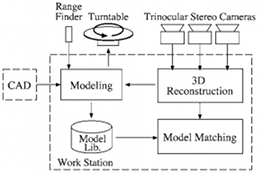
\includegraphics{figures/vvv}
\caption[Block diagram of VVV]{Block diagram of the ``VVV'' 3D vision robot system~\cite{sumi:2002}.}
\label{img:vvv}
\end{figure}

Another important contribution was given by Tomita \emph{et al.}~\cite{tomita:1998}: the Versatile 3D Vision system ``VVV'' can construct the 3D geometric data of any scene when two or more images are given, by using structural analysis and partial pattern matching. It can also recognize objects, although under the assumption that their geometric models are known. This is a relevant difference from our proposed approach, which, instead, is free of geometric models. A general user of VVV can make a task-oriented system whose ability is at least the same of a specialized robotic system (one that was built for a very specific action).

\bigskip

Within this chapter we will summarize the techniques that are related to the modules that compose our proposed architecture. Section~\ref{sec:segmentation} will outline the main image segmentation techniques existing in literature; Section~\ref{sec:stereopsis} will give a brief insight on stereo vision and 3D reconstruction; Section~\ref{sec:manipulation} will present the existing approaches for visual-based robot manipulator control; Section~\ref{sec:affordances} will introduce the object affordances learning tool, to improve manipulation performances.

%%%%%%%%%%%%%%%%
\section{Image Segmentation Techniques}
\label{sec:segmentation} \index{image segmentation}

The human eye is powerful because it is extremely \emph{versatile}: it can recognize objects nearly instantly, it can follow (track) their motion, recognize the mood of living beings from their facial expressions, decide when a circumstance is dangerous, compute the number and speed of objects, and more. It is because of this breadth of skills that the human eye is \emph{difficult to emulate}.

Recent \ac{CV} systems, on the other hand, are normally highly specialized; furthermore, they usually work well only under certain hypotheses. Some relevant fields of research inside \ac{CV} are tracking and image segmentation.

The purpose of image segmentation is to better organize the way we process a picture, by separating the interesting or relevant parts from those which are not useful for a given problem. Image segmentation, or simply ``segmentation''\index{segmentation|see{image segmentation}} for brevity, consists of dividing an image into two or more subset regions that cover it, according to a certain criterion, in order to simplify the representation and focus the attention on relevant parts of the image~\cite{foley}.

\begin{figure}
\centering
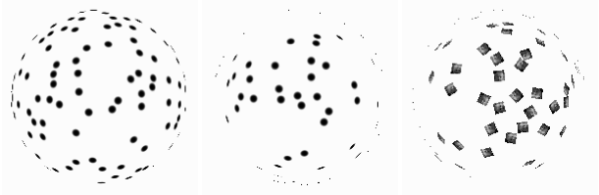
\includegraphics[scale=0.5]{figures/segm_3blobs}
\caption[Why segmentation is difficult]{Why segmentation is difficult: these are three surfaces whose image information can be organized into meaningful assemblies easily and successfully by the human eye, but it is not straightforward to do so for machines.}
%Picture: \cite{forsyth}.
\label{img:segment_3blobs}
\end{figure}

One of the major difficulties in object recognition problems is knowing \emph{which} pixels we have to recognize, and which to ignore~\cite{forsyth}. For example, it is difficult to tell whether a pixel lies on the surfaces in Fig.~\ref{img:segment_3blobs} simply by looking at the pixel. Specifically, it is difficult to tell whether a pixel lies on the three surfaces in the picture simply by looking at the pixel; the solution to the problem is to work with a \emph{compact representation} of the ``interesting'' image data that emphasize relevant properties. Segmentation is the process of obtaining such compact representation~\cite{shapiro_stockman}.

The goal in many tasks is for the regions to represent \emph{meaningful} areas of the image, such as crops, urban areas, and forests of a satellite image. Each of the resulting subsets contains those pixels of the image which satisfy a given condition: for instance, having the same colour, the same texture, or having rough edges. Furthermore, changing the representation of an image to something more meaningful means that it also becomes \emph{easier to analyze} and process.

Practical applications\index{image segmentation!applications} of image segmentation include:
\begin{itemize}
\item recognizing a face or any other trait that is \emph{salient} in a given situation;

\item traffic controlling systems;

\item medical imaging:
	\begin{itemize}
	\item[-] revealing, diagnosing and examining tumours;
	
	\item[-] studying other pathologies and anatomical structures;
		
	\item[-] measure the volume of tissues;
	
	\item[-] computer-guided surgery;
	\end{itemize}

\item locate objects in satellite images;

\item fingerprint recognition.
\end{itemize}

Traditionally~\cite[ch.~10]{shapiro_stockman}, segmentation has had two objectives:
\begin{enumerate}
\item to decompose the image into parts for further analysis;

\item to perform a change of representation.
\end{enumerate}

The importance of the first objective is straightforward to understand and is discussed thoroughly in texts like~\cite{foley, forsyth, shapiro_stockman, trucco_verri}. The second one, however, is more subtle: the pixels of an image must be organized into higher-level units that are either more meaningful or more efficient for further analysis, or both. A critical issue is whether or not segmentation can be performed for many different domains using bottom-up methods that do not use any special domain knowledge.

\bigskip

Since there is no general solution to the image segmentation\index{image segmentation} problem, several different approaches to implement segmentation have been proposed in literature, each having its advantages and drawbacks. A brief list of the most common techniques will now be given. Further down, the \ac{CAMSHIFT}\index{CAMSHIFT} algorithm, which belongs to the class of histogram-based\index{image segmentation!histogram-based} segmentation approaches (see~Section~\ref{sec:histo}) and is the technique adopted in this thesis, will be detailed.

%%%%%%%%%%%%%%%%
\subsection{Clustering Segmentation}
\index{image segmentation!clustering}

In pattern recognition, \emph{clustering} is the process of partitioning a set of pattern vectors into subsets called clusters~\cite{theodoridis}. Several types of clustering algorithms have been found useful in image segmentation. %These include classical clustering algorithms, simple histogram-based methods, Ohlander's recursive histogram-based technique, and more.

One way to look at the segmentation problem is thus to attempt to determine which components of a data set naturally ``belong together'' in a cluster. Generally, two approaches for clustering are considered in literature~\cite{forsyth}:

\begin{description}
\item[partitioning:] carving up a large data set according to some notion of the association between items inside the set, i.e., decomposing the set into pieces that are good with regards to a model. For example:
	\begin{itemize}
	\item[-] decomposing an image into regions that have coherent colour and texture inside them;
	
	\item[-] decomposing an image into extended blobs, consisting of regions that have coherent colour, texture and motion and look like limb segments;
	
	\item[-] decomposing a video sequence into shots---segments of video showing about the same scene from about the same viewpoint.
	\end{itemize}

\item[grouping:] starting from a set of distinct data items, collect sets of these items that make sense \emph{together} according to a model. Effects like occlusion mean that image components that belong to the same object are often separated. Examples of grouping include:
	\begin{itemize}
	\item[-] collecting together tokens that, when taken together, form a line;
	
	\item[-] collecting together tokens that seem to share a fundamental matrix.
	\end{itemize}
\end{description}

The key issue in clustering is to determine a suitable representation for the problem in hand.

\label{kmeans}
A famous clustering algorithm is $k$-Means\index{image segmentation!clustering!$k$-Means}, first described in~\cite{macqueen:1967}. Basic pseudocode is shown in Algorithm~\ref{algo:kmeans}. $k$-Means is an iterative technique to partition an image into $k$ clusters. The algorithm works by randomly selecting centroids, finding out which elements are closest to the centroid, then working out the mean of the points belonging to each centroid, which becomes the new centroid. Region membership is checked again, and the new centroids are computed again. This operation continues until there are no points that change their region membership.

\begin{algorithm}
\caption{Basic $k$-Means}
\label{algo:kmeans} \index{image segmentation!clustering!$k$-Means}
\begin{algorithmic}[1]
\STATE Place $k$ points into the space represented by the objects that are being clustered. These points represent initial group centroids.
\STATE Assign each object to the group that has the closest centroid.
\STATE When all objects have been assigned, recalculate the positions of the $k$ centroids. 
\STATE Repeat Steps 2 and 3 until the centroids no longer move. This produces a separation of the objects into groups from which the metric to be minimized can be calculated.
\end{algorithmic}
\end{algorithm}

While the $k$-Means algorithm is guaranteed to converge, it has a few drawbacks:
\begin{itemize}
\item it may occur that $k$-Means converges to a local, possibly not global, solution;

\item the algorithm is significantly sensitive to the initial randomly-selected cluster centres (to reduce this effect, one can execute $k$-Means multiple times, but this is costly);

\item basic $k$-Means relies on the assumption that the number of clusters $k$ is known in advance. Alternatives have been proposed to overcome this limitation of the initial setting, for example ``Intelligent $k$-Means''\index{image segmentation!clustering!Intelligent $k$-Means} by Mirkin~\cite[p.~93]{mirkin}.
\end{itemize}

% don't forget that EM is a variant of $k$-Means

%%%%%%%%%%%%%%%%
\subsection{Edge Detection Segmentation}
\label{sec:edge_det} \index{image segmentation!edge detection}

% [b]
\begin{figure}
\centering
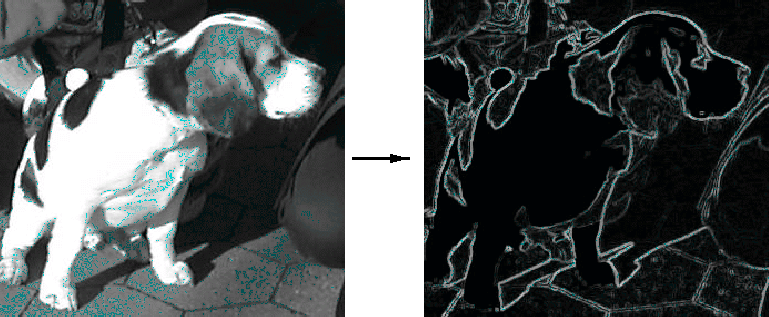
\includegraphics[scale=0.45]{figures/dog_edges}
\caption[Edge-based segmentation]{An example of edge-based segmentation, showing the computed edges of the left input image on the right.}
\label{img:dog_edges}
\end{figure}

\emph{Edge points}, or simply ``edges'', are pixels at or around which the image values undergo a sharp variation.

Edge detection techniques have been used as the base of several segmentation techniques, exploiting the tight relationship that exists between region boundaries and edges---the sharp adjustment in intensity at the region boundaries, as in Fig.~\ref{img:dog_edges}.

\begin{figure}
\centering
\subfloat[][A $325 \times 237$-pixel image, with scanline $i = 56$ (over the baby's forehead) highlighted.]
{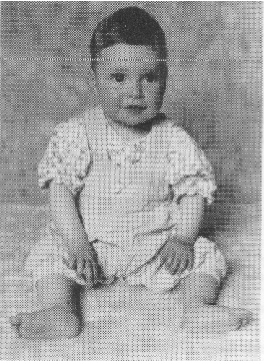
\includegraphics[width=.4\columnwidth]{figures/edge_baby} \label{fig:edge_baby} } \quad
% %necessary to prevent line break
\subfloat[][Intensity profile along the highlighted scanline.]
{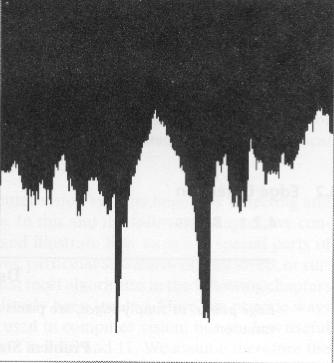
\includegraphics[width=.5\columnwidth]{figures/edge_baby_int} \label{fig:edge_baby_int} }

\caption[Edge detection and intensity profile]{An intensity image (left) and the intensity profile along a selected scanline (right). The main sharp variations correspond to significant contours.}
\label{fig:edge_det}
\end{figure}

The edge detection\index{image segmentation!edge detection} problem can be formulated like this: given an image that has been corrupted by acquisition noise, locate the edges most likely to be generated by scene elements (not by noise). Fig.~\ref{fig:edge_det} shows an example of edge detection computations.

Though, the edges identified by edge detection are often disconnected. To segment an object from an image, however, one needs closed region boundaries. Discontinuities are normally bridged if the distance between the two edges is within some predetermined threshold.

The Canny edge detection algorithm~\cite{canny:1986} \index{image segmentation!edge detection!Canny edge detection} is known as the optimal edge detector. It follows a list of three criteria with the aim of improving previous methods of edge detection:

\begin{description}
\item[good detection:] the algorithm should mark as many real edges in the image as possible. This is the first and most obvious principle, that of low error rate. It is important that edges occurring in images should not be missed and that there be no responses to non-edges.

\item[good localization:] the edges marked should be as close as possible to the edges in the real image. This second criterion suggests that the edge points should be well localized, in other words, that the distance between the edge pixels as found by the detector and the actual edge is to be at a minimum.

\item[minimal response:] a given edge in the image should only be marked once, and, where possible, image noise should not create false edges. The third criterion is thus to have only one response to a single edge; this was implemented because the first two criteria were not sufficient to completely eliminate the possibility of multiple responses to an edge.
\end{description}

To satisfy these requirements, the calculus of variations \index{calculus of variations} (a technique which finds the function which optimizes a given functional) is employed~\cite{canny:1986}. The optimal function in Canny's detector\index{image segmentation!edge detection!Canny edge detection} is described by the sum of four exponential terms, but can be approximated by the first derivative of a Gaussian. See Fig.~\ref{fig:canny} for an example.

\begin{figure}
\centering
\subfloat[][Input image: a colour photograph of a steam engine.]
{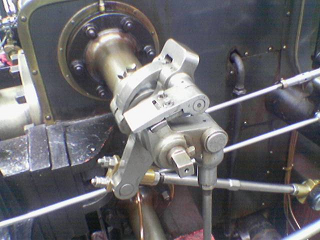
\includegraphics[width=.45\columnwidth]{figures/canny_valve_input} \label{fig:canny_valve_input} } \quad
%
\subfloat[][After having passed a $5 \times 5$ Gaussian mask across each pixel for noise reduction, the input image becomes slightly blurred.]
{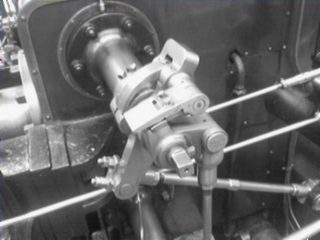
\includegraphics[width=.45\columnwidth]{figures/canny_valve_5pass} \label{fig:canny_valve_5pass} } \\
%
\subfloat[][Result of Canny edge detector.]
{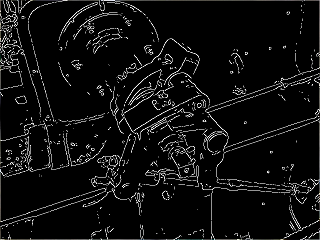
\includegraphics[width=.45\columnwidth]{figures/canny_valve_result} \label{fig:canny_valve_result} }
%
\caption[Canny edge detector]{Canny edge detector example.}
\label{fig:canny}
\end{figure}

%%%%%%%%%%%%%%%%
\subsection{Graph Partitioning Segmentation}
\index{image segmentation!graph partitioning}

Various algorithms exist in this class of methods, all of which model (groups of) pixels as vertices of a graph, while graph edges define the correlation or similarity among neighbouring pixels.

Popular graph partitioning segmentation techniques include: normalized cuts\index{image segmentation!graph partitioning!normalized cuts}, random walker, minimum mean cut, and minimum spanning tree-based algorithms.

Originally proposed by Shi and Malik~\cite{shi:1997}, the normalized cuts\index{image segmentation!graph partitioning!normalized cuts} method involves the modelling of the input image as a weighted, undirected graph. Each pixel is a node in the graph, and an edge is formed between every pair of pixels; the weight of an edge is a measure of the \emph{similarity} between the pixels.

The image is partitioned into disjoint sets (called ``segments''; see Fig.~\ref{img:norm_cuts}) by removing the edges that connect the segments. The optimal partitioning of the graph is the one that minimizes the weights of the edges that were removed (the ``cut''). The algorithm seeks to minimize the ``normalized cut''\index{image segmentation!graph partitioning!normalized cuts}, which is the ratio of the cut to all of the edges in the set.

\begin{figure}
\centering
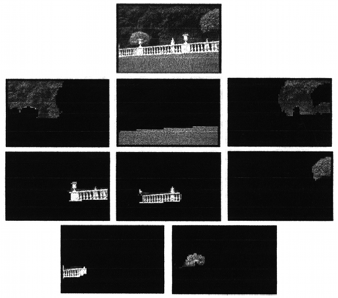
\includegraphics{figures/norm_cuts}
\caption[Graph partitioning segmentation: normalized cuts]{The image on top being segmented using the normalized cuts framework into the components shown below. The affinity measure used involved both intensity and texture. Thanks to having a texture measure, the railing shows as three reasonable coherent segments, which would not have happened with other approaches such as $k$-Means.}
\label{img:norm_cuts}
\end{figure}

%%%%%%%%%%%%%%%%
\subsection{Histogram-Based Segmentation}
\label{sec:histo} \index{image segmentation!histogram-based}

In this class of techniques, a histogram is computed from \emph{all} of the image pixels, taking into account colour or intensity values. Then, the peaks and valleys of such histogram are used to locate meaningful clusters in the image. By doing so, clusters are directly obtained after building the histogram.

See Fig.~\ref{img:colour_obj_tracking} for a generic scheme of these approaches. X, Y, and Area are relative to the colour probability distribution representing the tracked object (compare Section~\ref{sec:camshift_module}). Area is proportional to Z, i.e., the distance from the camera. Roll (inclination) is also tracked, as a fourth degree of freedom. For each video frame, the raw image is first converted to a colour probability distribution image via a colour histogram model of the colour being tracked (e.g., flesh for face tracking). The centre and size of the colour object are found via the \ac{CAMSHIFT}\index{CAMSHIFT} algorithm operating on the colour probability image. The current size and location of the tracked object are reported and used to set the size and location of the search window in the next video image. This process is iterated for continuous tracking.

Histogram-based segmentation\index{image segmentation!histogram-based} methods present an important advantage compared to other techniques: \emph{high efficiency}. Typically, these techniques require only one pass through the image pixels. For this reason, we will choose the \ac{CAMSHIFT}\index{CAMSHIFT}  algorithm, which belongs to this class, because we require a fast, simple, efficient tracker in our perceptual humanoid robotics framework.\index{perception}\index{humanoid robotics}

Building the histogram is a critical phase; as mentioned above, one can choose different types of measures like colour or intensity. This fact is important when envisioning a perceptual framework~\cite{bradski:1998}\index{PUI}, as is the case of our project and humanoid robotics.

\begin{figure}
\centering
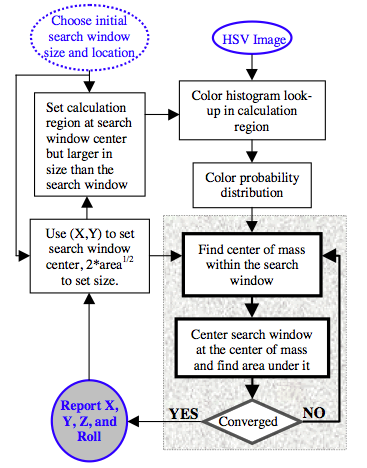
\includegraphics[scale=0.6]{figures/colour_obj_tracking}
\caption[Block diagram of object tracking]{Block diagram of histogram-based object tracking. The grey box is the Mean Shift\index{Mean Shift} algorithm.%
}
\label{img:colour_obj_tracking}
\end{figure}

A \ac{PUI} \index{PUI} is one in which a machine is given the ability to send and produce analogs of human senses, such as allowing computers to perceive\index{perception}\index{cognition} and produce localized sound and speech, giving robots a sense of touch and force feedback, or the ability to see.

% TODO: talk here about Mean Shift and CAMSHIFT?









%%%%%%%%%%%%%%%%
\subsection{Level Set Segmentation}
\label{sec:level_set} \index{image segmentation!level set}

In general, level set segmentation is a method for tracking the evolution of contours and surfaces. Originally proposed in~\cite{osher:1988}, this technique uses \ac{PSC}\index{PSC} schemes. The idea is to move surfaces under their curvature, propagating the surfaces towards the lowest potential of a cost function.

This framework has several advantages:
\begin{itemize}
\item level sets yield a useful representation of regions and their boundaries on the pixel grid without the need of complex (and costly) data structures. Therefore, optimization is simplified, as variational methods and standard numerics can be employed;

\item level sets can describe topological changes in the segmentation, i.e., parts of a region can split and merge;

\item it is possible to describe the image segmentation problem with a variational model, thus increasing flexibility (and permitting the introduction of additional features, shape knowledge, or joint motion estimation and segmentation).
\end{itemize}

\begin{figure}
\centering
\subfloat[][Input image.]
{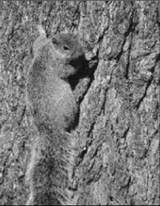
\includegraphics[width=.45\columnwidth]{figures/squirrel_ls1} \label{fig:squirrel_ls1} } \quad
% %necessary to prevent line break
\subfloat[][Level set segmentation.]
{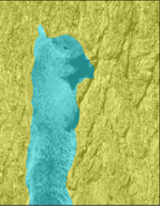
\includegraphics[width=.45\columnwidth]{figures/squirrel_ls2} \label{fig:squirrel_ls2} }
\caption[Level set segmentation]{Level set segmentation of a squirrel image: two regions have been detected.}
\label{fig:squirrel_ls}
\end{figure}

On the other hand, level set segmentation\index{image segmentation!level set} has a problem: a level set function is restricted to the separation of only two regions. Brox and Weickert~\cite{brox:2004} proposed a new formulation of the potential function to minimize, taking into account the number of regions, too.

\begin{figure}
\centering
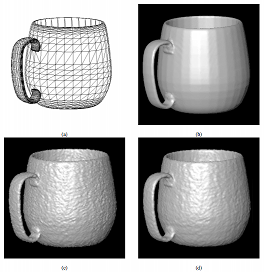
\includegraphics{figures/level_set_mug}
\caption[Level set based 3D reconstruction]{Level set based 3D reconstruction of a mug, using synthetic data generated from a 3D model~(a). Without noise, the reconstruction~(b) is limited only by the resolution of the model, $140 \times 140 \times 140$. With noise, the surface appears rough~(c). Including a prior improves the appearance of the reconstruction~(d).%
}
\label{img:level_set_mug}
\end{figure}

What is more, level set segmentation\index{image segmentation!level set} is well suited to generate 3D reconstructions\index{3D reconstruction} of objects~\cite{whitaker:1998}. See Fig.~\ref{img:level_set_mug} for a sample run of Whitaker's algorithm\index{image segmentation!level set!Whitaker's algorithm}. The strategy applied is as follows: construct a rather coarse volume that is the solution to a linear problem, i.e., the zero-level sets of a function, without the prior. This volume will serve as initialization for a level set model which moves towards the data given by range maps while undergoing a second-order flow to enforce the prior. After the rate of deformation slows to below some predefined threshold, the resolution is increased, the volume resampled, and the process repeated (in an attempt to avoid convergence to local minima).

Note that this last strategy employs predefined models of shapes: the approach has much to share with model-based segmentation methods, explained below.

%%%%%%%%%%%%%%%%
\subsection{Model-Based Segmentation}
\index{image segmentation!model-based}

Model-based segmentation approaches (or knowledge-based segmentation), commonly adopted in medical imaging\index{image segmentation!medical imaging}, rely on the assumption that structures of interest have a repetitive form of geometry.

State of the art methods in the literature for knowledge-based segmentation~\cite{freedman:2005} involve active shape and appearance models, active contours and deformable templates (see Fig.~\ref{img:model_based_prostate} for an example). Note that there is an intersection with level set segmentation methods\index{image segmentation!level set} (refer to Section~\ref{sec:level_set}).

One can seek a probabilistic model that explains the variation of the shape, for instance, of an organ and then, when segmenting an image, impose constraints using this model as a prior. Specifically, such a task involves:
\begin{enumerate}
\item registration\footnote{Registration fits models that are previously known; 3D reconstruction extracts models from images.}\index{registration} of the training examples to a common pose;

\item probabilistic representation of the variation of the registered samples; and

\item statistical inference between the model and the image.
\end{enumerate}

\begin{figure}
\centering
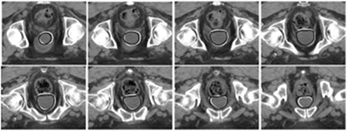
\includegraphics{figures/model_based_prostate}
\caption[Model based segmentation]{Model based segmentation results using a prostate model, to detect carcinoma cell masses. The white contour shows the result at convergence; the black contour shows the hand-drawn ground-truth contours supplied by a radiation oncologist.%
}
\label{img:model_based_prostate}
\end{figure}

So, these algorithms are based on matching probability distributions of photometric variables that incorporate learned shape and appearance models for the objects of interest. The main innovation is that there is no need to compute a pixel-wise correspondence between model and image. This allow for fast, principled methods.

%%%%%%%%%%%%%%%%
\subsection{Neural Networks Segmentation}
\index{image segmentation!neural networks}

Neural network image segmentation typically relies on processing \emph{small areas} of an image using an unsupervised neural network (a network where there is no external teacher affecting the classification phase) or a set of neural networks.

After such processing is completed, the decision-making mechanism marks the areas of an image accordingly to the category recognized by the neural network, as exemplified in Fig.~\ref{fig:nn_human_head}. A type of network well designed for these purposes~\cite{reyes:2000} is the Kohonen\index{Kohonen|see{\ac{SOM}}} \ac{SOM}\index{SOM}.

\begin{figure}
\centering
\subfloat[][Human head Magnetic Resonance input image.]
{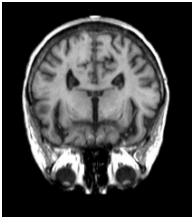
\includegraphics[width=.45\columnwidth]{figures/nn_human_head_input} \label{fig:nn_human_head_input} } \quad
%
\subfloat[][Neural Networks segmentation of MR image.]
{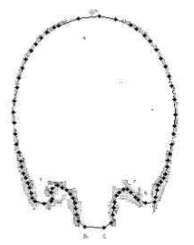
\includegraphics[width=.45\columnwidth]{figures/nn_human_head_segm} \label{fig:nn_human_head_segm} }
\caption{Neural Networks segmentation.}
\label{fig:nn_human_head}
\end{figure}

%%%%%%%%%%%%%%%%
\subsection{Region Growing Thresholding Segmentation}
\index{image segmentation!region growing}

Just like edge detection\index{image segmentation!edge detection} (see Section~\ref{sec:edge_det}) is implemented by quite different processes in photographs and range data, segmenting image into \emph{regions}\index{image segmentation!region growing}
 presents a similar situation.

Region growing is an approach to image segmentation in which neighbouring pixels are examined and added to a region class if no edges are detected~\cite{forsyth}. This process is iterated for each boundary pixel in the region. If adjacent regions are found, region-merging techniques are used in which weak edges are dissolved and strong edges are left intact.

This method offers several advantages over other techniques:
\begin{itemize}
\item unlike edge detection methods (such as gradient and Laplacian), the borders of regions found by region growing are thin --since one only adds pixels to the exterior of regions-- and connected;

\item the algorithm is stable with respect to noise: the resulting region will never contain too much of the background, as long as the parameters are defined correctly;

\item membership in a region can be based on multiple criteria, allowing us to take advantage of several image properties, such as low gradient or gray level intensity value, at once.
\end{itemize}

There are, however, disadvantages to region growing\index{image segmentation!region growing}. First and foremost, it is very \emph{expensive} computationally: it takes both serious computing power (processing power and memory usage) and a decent amount of time to implement and run the algorithms efficiently.

An example of region growing thresholding is~\cite{faugeras:1986}. This algorithm iteratively merges planar patches by maintaining a graph whose nodes are the patches and whose arcs (edges) are associated with their common boundary link adjacent patches. Each arc is assigned a cost, corresponding to the average error between the points of the two patches and the plane best fitting these points. The best arc is always selected, and the corresponding patches are merged. Note that the remaining arcs associated with these patches must be deleted while new arcs linking the new patch to its neighbors are introduced. The situation is illustrated by Fig.~\ref{img:region_growing}.

\begin{figure}
\centering
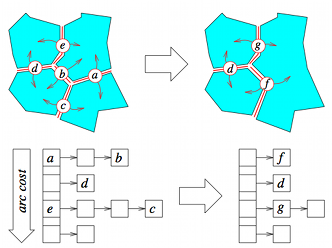
\includegraphics{figures/region_growing}
\caption[Region growing]{One iteration of the region growing process during which the two patches incident on the minimum-cost arc labelled $a$ are merged. The heap shown in the bottom part of the figure is updated as well (which bears a considerable computational cost): the arcs $a, b, c$ and $e$ are deleted, while two new arcs $f$ and $g$ are created and inserted in the heap.}
\label{img:region_growing}
\end{figure}

% this is a variant of the seeded region growing technique ->  requires the input of a number of seeds, either individual pixels or regions, which will control the formation of regions into which the image will be segmented
%One variant of this technique, proposed by Shapiro~\cite{shapiro_stockman}, is based on pixel intensities. The mean and scatter of the region and the intensity of the candidate pixel is used to compute a test statistic. If the test statistic is sufficiently small, the pixel is added to the region, and the region's mean and scatter are recomputed; otherwise, the pixel is rejected and it is used to form a new region.

%%%%%%%%%%%%%%%%
\subsection{Scale-Space Segmentation}
\index{image segmentation!scale-space}

Scale-space segmentation, also known as multi-scale segmentation, is based on the computation of image descriptors at multiple scales of smoothing. It is a general technique used for signal and image segmentation (see Fig.~\ref{img:scale-space_repr} and Fig.~\ref{img:scale-space_segm_ex}).

The main type of scale-space\index{image segmentation!scale-space} is the linear (Gaussian) scale-space, which has wide applicability as well as the attractive property of being possible to derive from a small set of scale-space axioms. The corresponding scale-space framework encompasses a theory for Gaussian derivative operators, which can be used as a basis for expressing a large class of visual operations for computerized systems that process visual information. This framework also allows visual operations to be made scale-invariant, which is necessary for dealing with the size variations that may occur in image data, because real-world objects may be of different sizes and in addition the distance between the object and the camera may be unknown and may vary depending on the circumstances.

For a two-dimensional image $f(x,y)$, its linear (Gaussian) scale-space \emph{representation} is a family of derived signals $L(x,y; t)$ defined by the convolution of $f(x,y)$ with the Gaussian kernel
\begin{equation}
g_t(x,y) = \frac{1}{2\pi t}e^{-(x^2 + y^2)/2t}
\end{equation}
such that
\begin{equation}
L(x,y; t) = (g_t * f)(x,y),
\end{equation}
where the semicolon in the argument of $L$ implies that the convolution is performed only over the variables $x,y$, while the scale parameter $t$ after the semicolon just indicates which scale level is being defined. This definition of $L$ works for a continuum of scales , but typically only a finite discrete set of levels in the scale-space representation would be considered.

\begin{figure}
\centering
\subfloat[][$t = 0$, corresponding to the original image $f$.]
{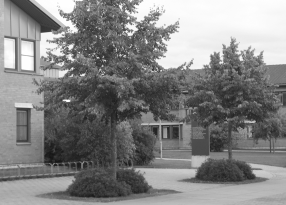
\includegraphics[width=.45\columnwidth]{figures/scale-space0} \label{img:scale-space0} } \quad
%
\subfloat[][$t = 1$.]
{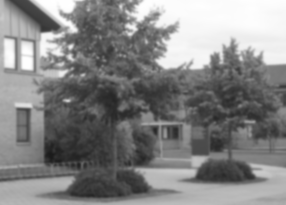
\includegraphics[width=.45\columnwidth]{figures/scale-space1} \label{img:scale-space1} } \\
\subfloat[][$t = 4$.]
{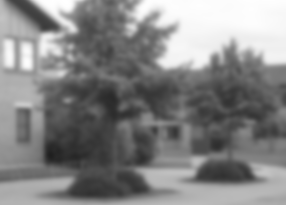
\includegraphics[width=.45\columnwidth]{figures/scale-space4} \label{img:scale-space4} } \quad
%
\subfloat[][$t = 16$.]
{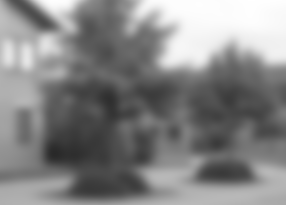
\includegraphics[width=.45\columnwidth]{figures/scale-space16} \label{img:scale-space16} }
%
\caption[Space-scale representation]{Space-scale representation $L(x,y; t)$ for various $t$ scales. As the parameter $t$ increases above $0$, $L$ is the result of smoothing $f$ with a larger and larger filter.}
\label{img:scale-space_repr}
\end{figure}

In Fig.~\ref{img:scale-space_dendro}, each ``x'' identifies the position of an extremum of the first derivative of one of 15 smoothed versions of the signal (red for maxima, blue for minima). Each ``+'' identifies the position that the extremum tracks back to at the finest scale. The signal features that persist to the highest scale (smoothest version) are evident as the tall structures that correspond to the major segment boundaries in the figure above.

\begin{figure}
\centering
\subfloat[][A signal (black), various multi-scale smoothed versions of it (red) and some segment averages (blue).]
{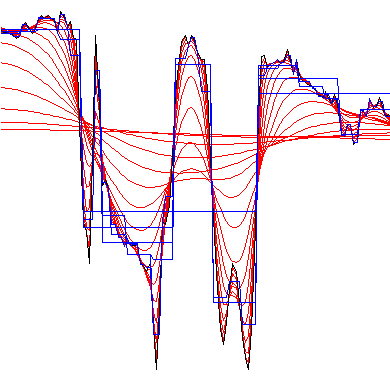
\includegraphics[width=.80\columnwidth]{figures/scale-space_segm} \label{img:scale-space_segm} } \\
%
\subfloat[][Dendrogram resulting from the segmentation in Fig.~\ref{img:scale-space_segm}.]
{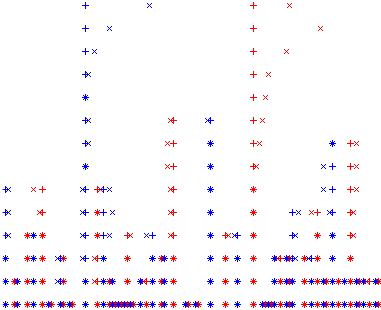
\includegraphics[width=.80\columnwidth]{figures/scale-space_dendro} \label{img:scale-space_dendro} }
\caption[Space-scale segmentation]{Space-scale segmentation example.}
\label{img:scale-space_segm_ex}
\end{figure}

%%%%%%%%%%%%%%%%
\subsection{Semi-Automatic Livewire Segmentation}
\index{image segmentation!semi-automatic}
\index{image segmentation!Livewire|see{image segmentation!semi-automatic}}

In this segmentation method, the user outlines the \ac{ROI} with mouse clicks, then an algorithm is applied so that the path that best fits the edge of the image is shown. It is based on the lowest cost path algorithm by Dijkstra\index{Dijkstra's algorithm}. 

The user sets the starting point clicking on an image pixel. Then, as he starts to move the mouse over other points, the smallest cost path is drawn from the starting point to the pixel where the mouse is over, changing itself if the user moves the mouse. If the user wants to choose the path that is being displayed, he will simply click the image again.

\begin{figure}
\centering
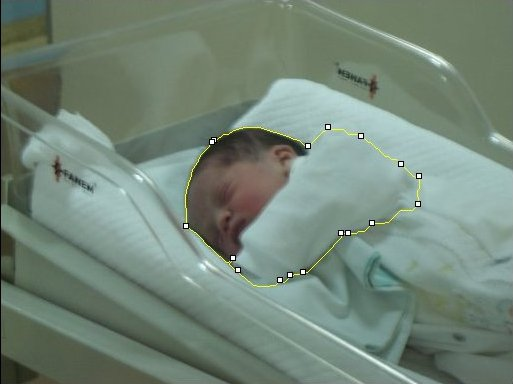
\includegraphics[scale=0.8]{figures/livewire_baby}
\caption[Semi-automatic Livewire segmentation]{Example run of a semi-automatic Livewire technique applied on a picture.}
\label{img:livewire_baby}
\end{figure}

One can easily see in Fig.~\ref{img:livewire_baby} that the places where the user clicked to outline the desired \ac{ROI} are marked with a small square. It is also easy to see that Livewire\index{image segmentation!semi-automatic} has snapped on the image borders.

% related technique: Intelligent Scissors

%%%%%%%%%%%%
%%%%%%%%%%%%
\section{Stereopsis}
\label{sec:stereopsis}
\index{stereopsis} \index{stereo vision|see{stereopsis}}

Since a considerable portion of this thesis work deals with how a humanoid robot can perceive object positions and orientations in 3D space by using a binocular head (see Section~\ref{sec:3d_recon_approach}), some introductory theoretical background is first due.

Stereopsis, also known as stereo vision or simply ``stereo'', allows two-dimensional images to be interpreted in terms of 3D scene structure and distance~\cite{trucco_verri}.

Humans have an uncanny ability to perceive and analyze the structure of the 3D world from visual input, operating effortlessly and with little or no idea of what the mechanisms of visual perception are.

Depending on the nature of the features we wish to observe (2D or 3D, points or lines on the surface of the object, etc.), different formulations and algorithms come into play. However, the underlying mathematics has much in common: all the different cases can be formulated in such a way that they require solutions of simultaneous transcendental, polynomial, or linear equations in multiple variables which represent the structure of the object and its 3D motion as characterized by rotation and translation.

\begin{figure}
\centering
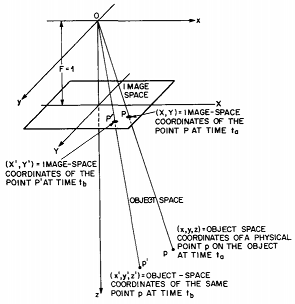
\includegraphics{figures/perspective_geom}
\caption[Perspective geometry for imaging]{Basic perspective geometry for imaging. Lower case letters refer to coordinates in the object space, upper case letters to coordinates on the image plane. Focal length (denoted here with $F$) is assumed to be $1$.}
\label{img:perspective_geom}
\end{figure}

In particular, what is inferred is a sensation of depth from the two slightly different projections of the world onto the retinas of the two eyes. The differences in the two retinal images are called horizontal disparity\index{horizontal disparity}, retinal disparity\index{retinal disparity|see{horizontal disparity}}, or binocular disparity\index{binocular disparity|see{horizontal disparity}}. The differences arise from the eyes' different positions in the head.

Stereo vision involves two processes:
\begin{itemize}
\item the binocular fusion of features observed by the two eyes;

\item the actual reconstruction of the features observed in the world.
\end{itemize}

They can be translated into two problems:
\begin{description}
\item[correspondence:]\index{correspondence} which parts of the left and right images are projections of the same scene element?

\item[reconstruction:]\index{3D reconstruction} given a number of corresponding parts of the left and right image, and possibly information on the geometry of the stereo system, what can we say about the 3D location and structure of the observed objects?
\end{description}

The correspondence problem is out of the scope of this project. In our proposed approach in Section~\ref{sec:3d_recon_approach}, we will focus on 3D reconstruction.

%%%%%%%%%%%%
%%%%%%%%%%%%
\section{Object Manipulation with Visual Servoing}\index{manipulation}
\label{sec:manipulation}

% which?
Existing visual-based robot control approaches~\cite{chaumette:visual1, chaumette:visual2, hutchinson:1996}, summarized below, solve the issue of representing a gripper--object relationship by handling \emph{models} of gripper and object in memory. This approach, while accurate and powerful, presents two drawbacks:
\begin{itemize}
\item the object model may be poor; besides, in several circumstances it may not be available at all (as addressed by Malis and Chaumette~\cite{malis:2002} or by Dufournaud \emph{et al.}~\cite{dufournaud:1998});

\item computational cost is high due to the manipulation program having to memorize and compute comparison operations to such models.
\end{itemize}

Visual Servoing~\cite{corke}\index{Visual Servoing} is a multi-disciplinary approach to the control of robots based on visual perception, involving the use of cameras to control the position of the robot relative to the environment as required by the task. This technique uses visual feedback information extracted from a vision sensor, to control the motion of robots. This discipline spans \ac{CV}, robotics, control, and real-time systems.

The task in Visual Servoing is to control the pose (3D position and orientation) of a robot's end-effector, using visual information (features) extracted from images.

Visual Servoing methods are commonly classified as image-based or position-based\footnote{Some ``hybrid approaches'' have also been proposed: 2-1/2-D Servoing, Motion Partition Based Servoing, and Partitioned DOF Based Servoing.}, depending on whether image features or the camera position define the signal error in the feedback loop of the control law.

\subsection{Image-Based Visual Servoing}
\index{Visual Servoing!Image-Based Visual Servoing}

\ac{IBVS} is a feature-based technique, meaning that it employs features that have been extracted from the image to directly provide a command to the robot (without any computation by the robot controller). Typically for \ac{IBVS}, all the information extracted from the image features and used in control, occurs in a 2D space. In most cases this coincides with the image coordinates' space. Despite this 2D information, because of which the approach is also known as ``2D servoing control'', the robot still has the capability to move in 3D.

\ac{IBVS} involves the estimation of the robot's velocity screw, $\dot{\mathbf{q}}$, so as to move the image plane features, ${\mathbf{f}}^c$, to a set of desired locations, ${\mathbf{f}}^*$~\cite{malis:2002}. \ac{IBVS} requires the computation of the \emph{image Jacobian} (or \emph{interaction matrix}). The image Jacobian represents the differential relationships between the scene frame and the camera frame (where either the scene or the camera frame is attached to the robot):
%
\begin{equation}
\mathbf{J}(\mathbf{q}) =
	\begin{bmatrix}
	\frac{\partial \mathbf{f}}{\partial \mathbf{q}}
	\end{bmatrix} =
	\begin{bmatrix}
	\frac{\partial f_1(\mathbf{q})}{\partial q_1} & \dots & \frac{\partial f_1(\mathbf{q})}{\partial q_m} \\
	\vdots & \ddots & \vdots \\
	\frac{\partial f_k(\mathbf{q})}{\partial q_1} & \dots & \frac{\partial f_k(\mathbf{q})}{\partial q_m}
	\end{bmatrix}
\end{equation}
%
where $\mathbf{q}$ represents the coordinates of the end-effector in some parameterization of the task space $\mathcal{T}$, $\mathbf{f} = [f_1, f_2, \dots, f_k]$ represents a vector of image features, $m$ is the cardinality of the task space $\mathcal{T}$, and $k$ is the number of image features.

\subsection{Position-Based Visual Servoing}
\index{Visual Servoing!Position-Based Visual Servoing}

\ac{PBVS} is traditionally a model-based technique. The pose of the object of interest is estimated with respect to the camera frame, then a command is issued to the robot controller, which in turn controls the robot. In this case, the image features are extracted as well, like in \ac{IBVS}, though the feature information is used to estimate the 3D object pose information in Cartesian space.

\begin{figure}
\centering
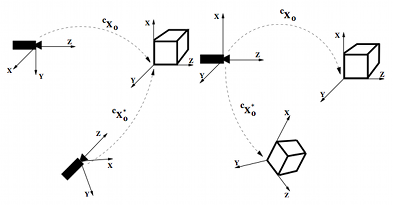
\includegraphics[scale=0.9]{figures/pbvs_examples}
\caption[Examples of \ac{PBVS}]{Two examples of \ac{PBVS} control. Left: eye-in-hand camera configuration, where the camera/robot is servoed from $\leftidx{^c}{\mathbf{x}}_0$ (current pose) to $\leftidx{^c}{\mathbf{x}}_0^*$ (desired pose). Right: a monocular, standalone camera system used to servo a robot-held object from its current to the desired pose.} 
\label{img:pbvs_examples}
\end{figure}

\ac{PBVS} is usually referred to as ``3D servoing control'', since image measurements are used to determine the pose of the target with respect to the camera and some common world frame. The error between the current and the desired pose of the target is defined in the task (Cartesian) space of the robot; hence, the error is a function of pose parameters, $\mathbf{e}(\mathbf{x})$. Fig~\ref{img:pbvs_examples} shows possible example tasks of \ac{PBVS}.

Fig~\ref{img:pbvs_block_diagram} illustrates the general working scheme of \ac{PBVS}, where the difference in pose between the desired and the current pose represents an \emph{error} which is then used to estimate the velocity screw for the robot, $\dot{\mathbf{q}} = [ \mathbf{V}; \mathbf{\Omega} ]^T$, in order to minimize that error.

\begin{figure}
\centering
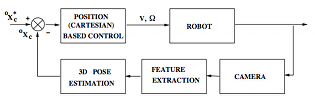
\includegraphics{figures/pbvs_block_diagram}
\caption[Block diagram of \ac{PBVS}]{Block diagram of \ac{PBVS}~\cite{hutchinson:1996}. The estimated pose of the target, $\leftidx{^c}{\mathbf{x}}_0$, is compared to the desired reference pose, $\leftidx{^c}{\mathbf{x}}_0^*$. This is then used to estimate the velocity screw, $\dot{\mathbf{q}} = [ \mathbf{V}; \mathbf{\Omega} ]^T$, for the robot so to minimize the error.}
\label{img:pbvs_block_diagram}
\end{figure}

%%%%%%%%%%%%
%%%%%%%%%%%%
\section{Object Affordances}
\label{sec:affordances}\index{object affordances}

Object affordances, or simply ``affordances'' for brevity, are a way to encode the relationships among actions, objects and resulting effects~\cite{montesano:2008}.

\begin{figure}
\centering
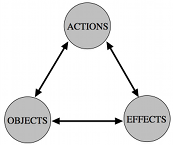
\includegraphics{figures/affordances}
\caption[Object affordances]{Object affordances represent the relationships that take place among actions (A), objects (O) and effects (E).}
\label{img:affordances}
\end{figure}

The general tool adopted to capture the dependencies in affordances (see Fig.~\ref{img:affordances}) is that of Bayesian networks\index{Bayesian networks}. Affordances make it possible to infer causality relationships by taking advantage of the intervention of a robot and the temporal ordering of events. Table~\ref{tab:affordances} lists the basic purposes of affordances.

\begin{table}
\caption[Purposes of object affordances]{Object affordances can be used for different purposes: to predict the outcome of an action, to plan the necessary actions to achieve a goal, or to recognize objects/actions.}
\label{tab:affordances}
\centering
\medskip
\begin{tabular}{*{3}{l}}
\toprule
input & output & function \\
\otoprule
$(O,A)$ & $E$ & predict effect \\
\midrule
$(O,E)$ & $A$ & action recognition and planning \\
\midrule
$(A,E)$ & $O$ & object recognition and selection \\
\bottomrule
\end{tabular}
\end{table}

Contrary to similar approaches, in the affordances framework the dependencies shown in Fig.~\ref{img:affordances} are \emph{not} known in advance (in which case we would learn a mapping between paris of actions and objects, or use supervised learning). Not assuming any prior knowledge on these dependencies, with affordances we try to infer the graph of the network directly from the exteroceptive and proprioceptive measurements. In addition, the affordances model allows the robot to tune the free parameters of the controllers.

This framework combines well with a developmental architecture whereby the robot incrementally develops its skills. In this sense, affordances can be seen as a bridge between
\begin{itemize}
\item sensory--motor coordination, and

\item world understanding and imitation.
\end{itemize}

Results on the learning and usefulness of object affordances for robots that use monocular vision (one camera only) are discussed in~\cite{montesano:2008}. With the (future) work of this thesis we intend to combine affordances with information obtained from stereo vision.